\documentclass[9pt,a4paper]{article}

% --- Paquetes Esenciales ---
\usepackage{ifxetex}
\ifxetex
  \usepackage{fontspec}
  \setmainfont{Arial}
\else
  \usepackage[utf8]{inputenc}
  \usepackage[T1]{fontenc}
\fi
\usepackage[spanish,es-tabla]{babel}
\usepackage[top=1.2cm, bottom=1.25cm, left=1.55cm, right=1.55cm, headheight=11pt]{geometry}
\usepackage{amsmath, amssymb}
\usepackage{booktabs}
\usepackage{tabularx}
\usepackage{graphicx}
\usepackage{xcolor}
\usepackage{enumitem}
\usepackage{fancyhdr}
\usepackage[colorlinks=true, linkcolor=blue!75!black, citecolor=blue!75!black, urlcolor=blue!75!black]{hyperref}

% --- Paleta de Colores Institucional ---
\definecolor{whrmagenta}{HTML}{9D174D}
\definecolor{gallupgreen}{HTML}{065F46}
\definecolor{darkslate}{HTML}{0F172A}
\definecolor{softslate}{HTML}{334155}
\definecolor{lightbg}{HTML}{F8FAFC}

% --- Configuración de Párrafos y Espaciado ---
\setlength{\parskip}{0.14em}
\setlength{\parindent}{0pt}
\setlist{nosep, leftmargin=1.1em, topsep=0.5pt, partopsep=0pt, parsep=0pt, itemsep=0.8pt}

% --- Encabezado y Pie de Página ---
\pagestyle{fancy}
\fancyhf{}
\renewcommand{\headrulewidth}{0.3pt}
\renewcommand{\footrulewidth}{0.3pt}
\lhead{\scriptsize\textcolor{softslate}{\textbf{Proyecto 2 · Visualización I} --- World Happiness Report 2024}}
\rhead{\scriptsize\textcolor{whrmagenta}{\textbf{Informe Analítico y Resumen Ejecutivo}}}
\lfoot{\scriptsize\textcolor{softslate}{Maestría / Pregrado en Ciencia de Datos · Adriana Pineda, Paola Moreno}}
\rfoot{\scriptsize\textcolor{softslate}{\textbf{Página \thepage\ de 3}}}

% --- Comandos de Encabezados Compactos ---
\newcommand{\customsection}[1]{%
  \vspace{0.2em}%
  {\small\bfseries\color{whrmagenta}#1}%
  \vspace{0.05em}\par%
}
\newcommand{\customsubsection}[1]{%
  \vspace{0.15em}%
  {\footnotesize\bfseries\color{darkslate}#1}%
  \vspace{0.04em}\par%
}

\begin{document}

% ==============================================================================
% PÁGINA 1: CONTEXTO, AUDIENCIA, PREGUNTA Y DATOS
% ==============================================================================

\begin{center}
    {\normalsize\bfseries\color{darkslate} Bienestar entre Países: ¿En qué Dimensiones se Separan las Naciones con Mayor y Menor Evaluación de Vida?}\\[0.15em]
    {\scriptsize\textcolor{whrmagenta}{\textbf{Informe Analítico Ejecutivo, Caracterización de Brechas Cuartílicas y Descomposición Empírica}}}\\[0.2em]
    {\scriptsize\textbf{Equipo de Trabajo:} Arnold Santiago Torres Anzola \quad|\quad Juan David Cruz Romero}\\[0.08em]
    {\tiny\textcolor{softslate}{Curso: Visualización I --- Docentes: Adriana Pineda, Paola Moreno --- Convención: \texttt{EquipoX\_Proyecto2\_Resumen.pdf}}}
\end{center}

\vspace{-0.4em}
\hrule height 0.5pt
\vspace{0.15em}

\customsection{1. Audiencia Técnica Específica y Contexto Institucional}
\textbf{Destinatario:} El informe está dirigido al \textbf{Equipo Técnico de Análisis Comparativo de Bienestar y Políticas Públicas de un Organismo Multilateral de Desarrollo} (homólogo a la Unidad de Estadísticas del PNUD o la Dirección de Bienestar de la OCDE).

\textbf{Interés y necesidad analítica:} Este grupo de investigadores cuantitativos y científicos de datos evalúa diagnósticos comparativos internacionales para discernir \textit{en qué condiciones específicas se fragmenta la calidad de vida} entre las naciones más prósperas y las más rezagadas. Si las diferencias se concentraran primordialmente en el PIB per cápita, los diagnósticos y programas podrían limitarse al seguimiento macroeconómico; si, por el contrario, la brecha responde con igual o mayor intensidad a condiciones socioinstitucionales (redes de auxilio social, libertad de elección o probidad pública), el equipo técnico deberá incorporar obligatoriamente estas condiciones en sus recomendaciones de política pública.

\textbf{Expectativas de la audiencia:} Definiciones operativas transparentes, criterios reproducibles de agregación, trazabilidad completa de transformaciones, tratamiento documentado de valores faltantes y rigurosa \textit{cautela inferencial}, evitando atribuir causalidad a datos de naturaleza observacional y transversal.

\customsection{2. Planteamiento del Problema y Pregunta Analítica Central}
Las evaluaciones de calidad de vida presentan una profunda heterogeneidad internacional, con brechas que superan los 6 puntos en la escala de Cantril entre las naciones más favorecidas y aquellas sumidas en crisis humanitarias. Para orientar el análisis, se formula la siguiente pregunta central:

\vspace{0.1em}
\begin{center}
\colorbox{lightbg}{\parbox{0.98\textwidth}{%
\footnotesize\bfseries\textcolor{darkslate}{«¿En qué dimensiones del bienestar (económica, de salud y socioinstitucional) se observan las mayores diferencias entre los países con mayor y menor evaluación de vida en el World Happiness Report 2024, y qué países se apartan del patrón observado?»}%
}}
\end{center}
\vspace{0.1em}

\textbf{Subpreguntas y objetivos:} (1) ¿En qué condiciones específicas (económica, salud, socioinstitucional) se concentran las mayores brechas absolutas entre cuartiles extremos ($Q4$ vs. $Q1$)? (2) ¿En qué medida el ingreso por habitante es suficiente por sí solo para explicar los niveles de bienestar, o qué papel amortiguador desempeñan las redes de apoyo social y la confianza institucional? (3) ¿Qué naciones logran evaluaciones de vida significativamente superiores o inferiores a lo predicho por su ingreso, y qué factores explican dicha divergencia?

\customsection{3. Descripción del Conjunto de Datos y Preparación Documentada}
\textbf{Fuente oficial única:} Archivo mandatorio \texttt{WHR24\_Data\_Figure\_2.1.xls} (World Happiness Report 2024), que consolida el promedio móvil trienal nacional para el periodo 2021--2023, ordenando a 143 países en 11 columnas.

\textbf{Variable objetivo (dependiente):} \textit{Ladder score} (escalera de Cantril, 0 a 10), un instrumento psicométrico de la encuesta mundial de Gallup donde 0 representa la peor vida posible y 10 la mejor vida alcanzable. Incluye sus límites al 95\% de confianza (\texttt{lowerwhisker}, \texttt{upperwhisker}).

\textbf{Descomposición aditiva econométrica:} El archivo no registra los indicadores en sus unidades brutas originales, sino la \textit{porción de la evaluación de vida de cada país que el modelo de regresión asocia con cada indicador}, expresada en puntos de la escalera de Cantril y respecto a un país teórico denominado \textit{Distopía} (referente hipotético con los valores mínimos observados internacionalmente, aporte base $\approx 1.97$ pts). Por diseño del reporte, las seis contribuciones modeladas más el residuo no explicado (\texttt{Dystopia + residual}) suman exactamente el \textit{Ladder score}:
\begin{equation*}
\footnotesize
\text{Ladder score}_i = \text{PIB}_i + \text{ApoyoSocial}_i + \text{Salud}_i + \text{Libertad}_i + \text{Generosidad}_i + \text{Corrupción}_i + (\text{Distopía + residuo})_i
\end{equation*}

\vspace{-0.3em}
\textbf{Criterio de segmentación cuartílica (25\% extremos):} Para comparar grupos contrastantes de forma reproducible y balanceada, se definen dos cuartiles empíricos de 36 países cada uno ($N=143$):
\begin{itemize}
    \item \textbf{Cuartil Superior ($Q4$ - Alto Bienestar):} Países con $\text{Ladder score} \ge 6.416$ pts (36 naciones; desde Finlandia: 7.741 hasta España: 6.421 pts; media = 6.88 pts).
    \item \textbf{Cuartil Inferior ($Q1$ - Bajo Bienestar):} Países con $\text{Ladder score} \le 4.726$ pts (36 naciones; desde Pakistán: 4.657 hasta Afganistán: 1.721 pts; media = 3.91 pts).
    \item \textbf{Segmento Central ($Q2-Q3$):} 71 naciones con bienestar intermedio (mediana global = 5.79 pts; media = 5.53 pts).
\end{itemize}

\textbf{Tratamiento de casos especiales y valores faltantes:}
\begin{itemize}
    \item \textit{Faltantes en descomposición ($n = 140$):} Baréin, Tayikistán y Estado de Palestina tienen \textit{Ladder score} pero no registran contribuciones explicativas. Se incluyen en los cuartiles agregados pero se excluyen de los análisis por dimensiones ($n = 140$).
    \item \textit{Ajustes de regresión MCO:} Venezuela registra aporte de $\text{PIB} = 0.000$ (se excluye de la estimación de la recta lineal económica para evitar distorsiones contables). Líbano registra un valor atípico de \textit{Distopía + residuo} negativo ($-0.073$ pts), reflejo de un colapso multidimensional severo.
\end{itemize}

\clearpage

% ==============================================================================
% PÁGINA 2: PRINCIPALES HALLAZGOS E INTERPRETACIÓN DE VISUALIZACIONES
% ==============================================================================

\customsection{4. Principales Hallazgos Empíricos e Interpretación de Visualizaciones (Numeral 8)}

La Tabla~\ref{tab:brechas} sintetiza la descomposición cuantitativa de la brecha total de \textbf{+2.96 puntos} entre los promedios de $Q4$ y $Q1$. La Figura~\ref{fig:resumen} expone la magnitud estandarizada de cada componente (A) y la articulación econométrica del bienestar frente al tejido socioinstitucional (B).

\begin{table}[h!]
\centering
\scriptsize
\renewcommand{\arraystretch}{0.84}
\setlength{\tabcolsep}{3pt}
\caption{Matriz comparativa de contribuciones promedio por cuartil y descomposición de la brecha $Q4 - Q1$.}
\label{tab:brechas}
\vspace{0.1em}
\begin{tabularx}{\textwidth}{lccccc}
\toprule
\textbf{Componente / Dimensión Analítica} & \textbf{Q1 (Bajo, pts)} & \textbf{Q4 (Alto, pts)} & \textbf{Brecha (pts)} & \textbf{Brecha ($z$)} & \textbf{¿Traslape Empírico $Q1-Q4$?} \\
\midrule
PIB per cápita (Dimensión Económica) & 0.92 & 1.82 & \textbf{+0.90} & 3.9 desv. est. & Sí ($[0.53, 1.45]$ vs $[1.27, 2.14]$) \\
Apoyo social (Dimensión Socioinstitucional) & 0.74 & 1.41 & \textbf{+0.67} & 3.1 desv. est. & Sí ($[0.00, 1.28]$ vs $[1.08, 1.62]$) \\
Esperanza de vida saludable (Dimensión Salud) & 0.35 & 0.66 & \textbf{+0.32} & 3.2 desv. est. & Sí ($[0.00, 0.59]$ vs $[0.51, 0.77]$) \\
Libertad para decidir (Socioinstitucional) & 0.49 & 0.74 & \textbf{+0.25} & 1.8 desv. est. & Sí ($[0.00, 0.86]$ vs $[0.53, 0.86]$) \\
Probidad pública / Percepción de corrupción & 0.12 & 0.29 & \textbf{+0.17} & 1.5 desv. est. & Sí ($[0.01, 0.26]$ vs $[0.01, 0.57]$) \\
\midrule
\textbf{Suma Socioinstitucional (Apoyo + Libertad + Probidad)} & \textbf{1.35} & \textbf{2.44} & \textbf{+1.09} & \textbf{3.5 desv. est.} & \textbf{No (Casi nulo: máx. $1.953$ vs mín. $1.959$)} \\
Generosidad (Comportamiento prosocial) & 0.15 & 0.17 & +0.02 & 0.2 desv. est. & Sí (Prácticamente no discrimina) \\
Distopía + residuo (Componente no modelado) & 1.15 & 1.79 & +0.65 & 1.3 desv. est. & Sí (Peso relevante: 22.0\% de la brecha) \\
\midrule
\textbf{Evaluación Global de Vida (Ladder score)} & \textbf{3.91} & \textbf{6.88} & \textbf{+2.96} & \textbf{4.2 desv. est.} & \textbf{No (Segmentación por definición)} \\
\bottomrule
\end{tabularx}
\end{table}

\vspace{-0.65em}

\begin{figure}[h!]
\centering
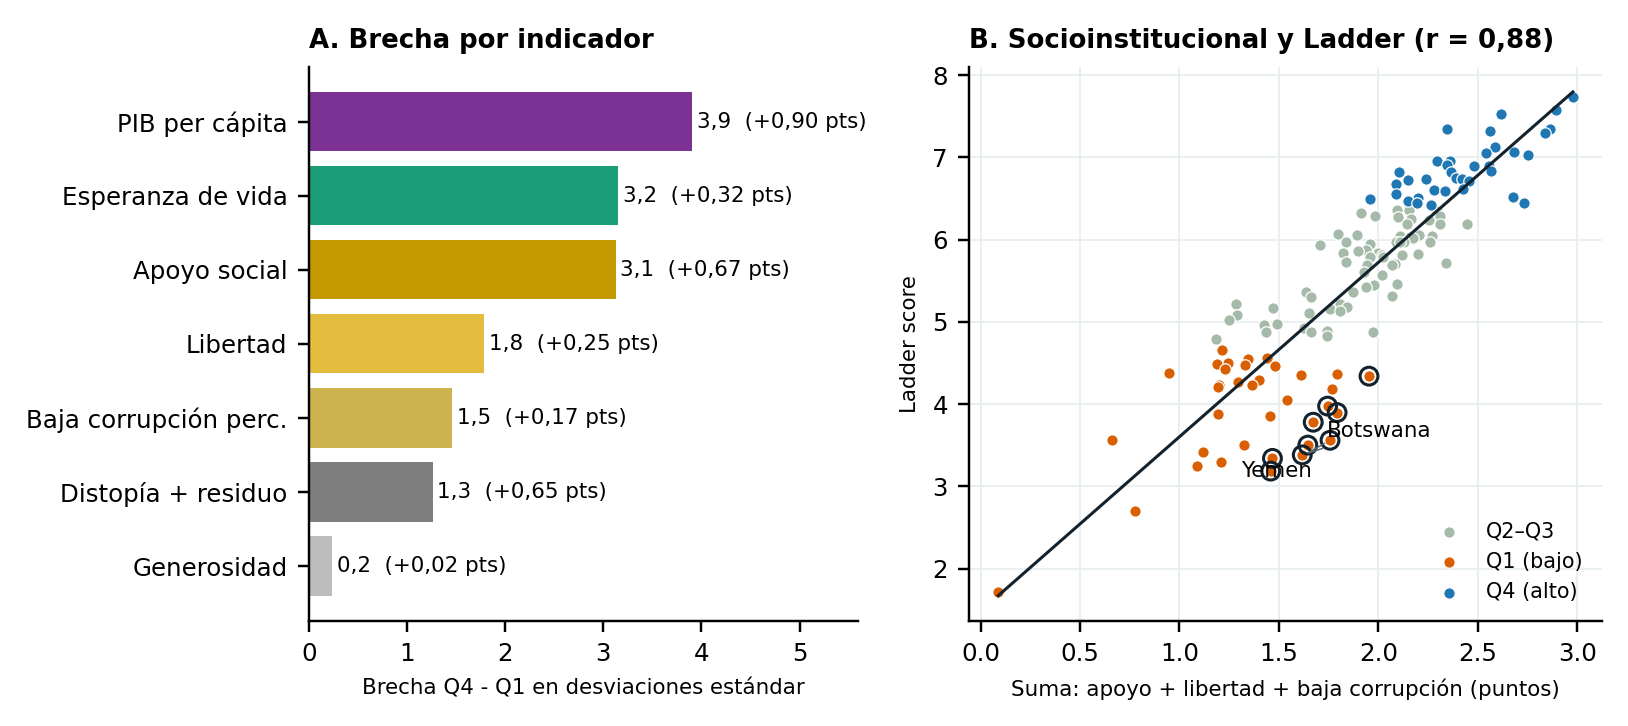
\includegraphics[width=0.64\textwidth]{figura_resumen_brechas.png}
\vspace{-0.35em}
\caption{\scriptsize \textbf{(A)} Brecha estandarizada $Q4 - Q1$ por indicador (entre paréntesis, diferencia en puntos de la escala). \textbf{(B)} Ajuste econométrico MCO entre Dimensión Socioinstitucional y Ladder score ($r=0.88, n=140$), destacando países atípicos y separación de cuartiles.}
\label{fig:resumen}
\end{figure}

\vspace{-0.8em}

\customsubsection{Interpretación Rigurosa de Patrones, Comparaciones y Relaciones}
\begin{itemize}[leftmargin=1.1em]
    \item \textbf{La condición económica explica la mayor brecha individual (+0.90 pts):} El PIB per cápita representa el \textbf{30.4\% de la distancia total} entre cuartiles ($+0.90$ de $+2.96$ pts), alcanzando $3.9$ desviaciones estándar. La capacidad económica es un predictor primario indispensable del bienestar colectivo ($r = 0.80$ con $R^2 = 0.64$, $n=139$), pero deja un 36\% de varianza que la economía sola no acompaña.
    \item \textbf{La dimensión socioinstitucional supera al ingreso en peso acumulado (+1.09 pts):} Al consolidar las tres variables del entorno social (apoyo comunitario $+0.67$, libertad vital $+0.25$ y probidad $+0.17$), la brecha agregada asciende al \textbf{36.8\% del diferencial global} ($+1.09$ pts). Su asociación lineal con el \textit{Ladder score} es aún más estrecha ($r = 0.88, n=140$) que la del PIB. A diferencia de las variables aisladas (donde siempre hay traslape), en la suma socioinstitucional $Q1$ llega hasta $1.953$ (Camboya) y $Q4$ inicia en $1.959$ (Rumania), configurando una separación empírica casi nítida entre ambos mundos.
    \item \textbf{Salud física como factor intermedio prioritario (+0.32 pts):} La esperanza de vida saludable genera una brecha sustantiva de $3.2$ desviaciones estándar ($10.8\%$ de la distancia total), confirmando que la longevidad libre de discapacidad es un requisito funcional del bienestar humano.
    \item \textbf{Generosidad como factor no discriminante (+0.02 pts):} Con apenas $+0.02$ pts ($0.2$ desv. est.), la solidaridad monetaria ocurre tanto en países de ingreso alto como de ingreso bajo, careciendo de capacidad explicativa para segmentar los niveles de desarrollo internacional.
    \item \textbf{Magnitud crítica del residuo no explicado (+0.65 pts):} La brecha en \textit{Distopía + residuo} explica el \textbf{22.0\% de la divergencia total}. Esto evidencia que más de una quinta parte de la brecha obedece a factores estructurales no capturados por las seis variables del modelo (conflictos bélicos, colapso de seguridad ciudadana o factores culturales locales).
    \item \textbf{Casos atípicos de resiliencia comunitaria frente a colapso institucional:} El análisis de residuos MCO sobre el ingreso y la dimensión socioinstitucional revela profundas asimetrías de interés para estudios de caso:
    \begin{itemize}[nosep]
        \item \textit{Resiliencia comunitaria (por encima de la recta):} Naciones como \textbf{Nicaragua} ($+1.43$ pts de residuo), \textbf{El Salvador} ($+1.22$ pts), \textbf{Costa Rica} y \textbf{Mozambique} ($+1.61$ pts) compensan un PIB per cápita moderado o bajo mediante redes densas de apoyo familiar y respaldo social, logrando evaluaciones vitales muy superiores a las que sugeriría su ingreso.
        \item \textit{Vulnerabilidad y déficit cívico (por debajo de la recta):} En contraste, naciones de ingreso medio-alto como \textbf{Botsuana} ($-2.28$ pts respecto a su PIB; aporte PIB $= 1.445$ vs apoyo social $= 0.969$) y \textbf{Líbano} ($-2.80$ pts; colapso institucional y residuo Distopía negativo) presentan evaluaciones de vida que se desploman debido a la fractura del capital social, la desconfianza institucional y crisis prolongadas. En ambos casos, el intervalo de confianza al 95\% del \textit{Ladder score} excluye la recta, confirmando anomalías estructurales y no meros errores muestrales.
    \end{itemize}
\end{itemize}

\clearpage

% ==============================================================================
% PÁGINA 3: CONCLUSIONES, LIMITACIONES, PLATAFORMA Y ANEXO IA
% ==============================================================================

\customsection{5. Conclusiones y Respuestas a la Pregunta Analítica (Numeral 9)}

En respuesta directa y fundamentada a la pregunta central formulada para la audiencia técnica de políticas públicas:

\begin{enumerate}[leftmargin=1.15em, itemsep=0.2em]
    \item \textbf{El ingreso económico es condición necesaria pero no suficiente:} El PIB per cápita representa la mayor brecha individual ($+0.90$ pts, $30.4\%$ del total). Sin embargo, un enfoque que concentre las recomendaciones de política exclusivamente en el crecimiento económico generará diagnósticos incompletos, pues la economía sola no garantiza bienestar elevado cuando coexisten fracturas en el tejido social.
    \item \textbf{El capital socioinstitucional constituye el principal divisor del bienestar humano (+1.09 pts):} La concurrencia de apoyo social, libertad para tomar decisiones de vida y probidad pública explica el $36.8\%$ de la brecha entre cuartiles. La solidez de estas redes comunitarias es lo que permite a ciertas economías emergentes alcanzar niveles de bienestar equiparables a los de Europa, mientras que su ausencia precipita a países de ingreso medio a los peldaños más bajos de la escala global.
    \item \textbf{Relevancia del seguimiento a casos atípicos:} La identificación cuantitativa de naciones con residuo estandarizado $|z| \ge 2.0$ proporciona una guía prioritaria para estudios de caso: naciones resilientes ofrecen lecciones sobre preservación de cohesión social, mientras que naciones rezagadas alertan sobre crisis de gobernanza y aislamiento relacional.
\end{enumerate}

\customsection{6. Reconocimiento de Limitaciones Metodológicas}
\begin{itemize}[leftmargin=1.1em, itemsep=0.1em]
    \item \textbf{Asociación observacional sin causalidad:} Todas las inferencias describen correlaciones y descomposiciones estadísticas a nivel agregado de país. No es metodológicamente válido interpretar que un incremento en un componente producirá mecánicamente un aumento causal en el bienestar de la población.
    \item \textbf{Identidad aditiva intrínseca al modelo:} Como las seis variables explicativas y \textit{Distopía + residuo} se estiman para reproducir el \textit{Ladder score}, su asociación con el puntaje está parcialmente determinada por la construcción econométrica oficial del WHR 2024.
    \item \textbf{Falta de desagregación sociodemográfica:} El archivo \texttt{WHR24\_Data\_Figure\_2.1.xls} no provee datos desagregados por sexo, edad, etnia ni territorio subnacional, ocultando posibles desigualdades distributivas al interior de cada país.
    \item \textbf{Sensibilidad a los umbrales cuartílicos:} El criterio del 25\% es objetivo y reproducible, pero otros umbrales (quintiles o deciles) podrían modular sutilmente los valores absolutos de las brechas.
\end{itemize}

\customsection{7. Plataforma Interactiva Oficial y Recursos Reproducibles}
En cumplimiento estricto de los requisitos del proyecto, se desarrollaron dos artefactos reproducibles complementarios:
\begin{itemize}[leftmargin=1.1em, itemsep=0.1em]
    \item \textbf{Cuaderno Jupyter Reproducible:} \texttt{notebooks/EquipoX\_Proyecto2\_Visualizacion.ipynb}, estructurado en 6 visualizaciones (4 estáticas en Seaborn y 2 interactivas en Plotly), ejecutable integralmente sin errores de principio a fin.
    \item \textbf{Plataforma Web Interactiva Oficial WHR / Gallup Analytics:} \texttt{exports/EquipoX\_Proyecto2\_Dashboard.html}, portal interactivo desarrollado con la identidad visual oficial del \textit{World Happiness Report} y paleta Gallup (\texttt{\#E0288A} y \texttt{\#008559}). Integra 4 módulos navegables (\textit{Map}, \textit{Chart}, \textit{Rankings} y \textit{Variables \& Metodología}), buscador predictivo por país con autocompletado en tiempo real, filtro sincrónico por cuartiles y fichas técnicas modales.
\end{itemize}

\customsection{8. Anexo Técnico: Declaración de Uso de Inteligencia Artificial (Entregable 5)}
\begin{itemize}[leftmargin=1.1em, itemsep=0.1em]
    \item \textbf{Herramientas y Modelos Utilizados:} Modelos de lenguaje avanzados (Google Antigravity / Gemini 3.8 Flash).
    \item \textbf{Propósitos Específicos:}
    \begin{enumerate}[label=(\alph*), nosep]
        \item Optimización y depuración sintáctica de rutinas de preparación de datos y parametrización gráfica en \texttt{Seaborn} y \texttt{Plotly}.
        \item Calibración de accesibilidad cromática bajo normas WCAG para daltonismo (paletas azul petróleo \texttt{\#1F78B4} para $Q4$, terracota cálido \texttt{\#D95F02} para $Q1$ y neutros en escala de grises).
        \item Asistencia en la estructuración de ecuaciones algebraicas y diagramación tipográfica en \LaTeX{} para garantizar el límite estricto de 3 páginas.
    \end{enumerate}
    \item \textbf{Prompts Principales Empleados:}
    \textit{«Proporciona una paleta de colores cualitativa accesible (colorblind-safe) para contrastar dos cuartiles extremos y una categoría intermedia neutra en Seaborn y Plotly.»} \quad|\quad \textit{«Genera una rutina reproducible en Python para comprobar algebraicamente la identidad aditiva de las seis contribuciones explicadas y el término Distopía frente al Ladder score oficial del WHR 2024.»}
    \item \textbf{Reflexión Crítica sobre la Supervisión Humana:} Todos los algoritmos, estimaciones paramétricas e interpretaciones textuales generados fueron exhaustivamente contrastados, validados y ajustados por los integrantes del equipo frente al archivo oficial \texttt{WHR24\_Data\_Figure\_2.1.xls}, asegurando el rigor inferencial, la pertinencia institucional y la completa reproducibilidad técnica.
\end{itemize}

\end{document}
